\chapter{Экспериментальный раздел}
\label{cha:research}
    В данном разделе будут проведены эксперименты для проведения 
    сравнительного анализа алгоритмов по затрачиваемому процессорному 
    времени.

    \section{Сравнительный анализ на основе замеров времени работы алгоритмов}
        В рамках данного проекта были проведёны следующие эксперименты:

        1) сравнение нерекурсивных алгоритмов поиска расстояния Левенштейна и Дамерау-Левенштейна
        на строках длиной от 5 до 10 с шагом 1 (график \ref{graph:test:1});
        
        2) сравнение рекурсивного алгоритма поиска расстояния Дамуерау-Левенштейна и рекурсивного алгоритма Дамерау-Левенштейна с кэшированием на строках длиной от 0 до 12 с шагом 1 (график \ref{graph:test:2}).
        
        Тестирование проводилось на компьютере с процессором
        Intel(R) Core(TM) i5-8265U CPU @ 1.60GHz 1.80 GHz под управлением Windows 11 с 8 Гб оперативной памяти.\\

        Ниже представлены результаты замеров (таблица \ref{table:time}) для всех 4 алгоритмов \footnote{Прочерк в таблице означает, что для заданных значений тестирование не проводилось}.\\


\begin{table}[h]
	\begin{center}
		\caption{\label{table:time} Замеры времени (в секундах) для строк различной длины}
		\begin{tabular}{|c c c c c|} 
			\hline
			Длина строк & Л. матричный & Д.Л. матричный & Д.Л. рекурсивный & Д.Л. с кэшем\\ [0.5ex] 
			\hline\hline
			5 & 2.5e-0.5 & 0.002 & 5.3e-05 & 0.003\\
			\hline
			6 & 3.4e-0.5 & 0.009 & 6.7e-05 & 0.015\\
			\hline
			7 & 4.3e-0.5 & 0.031 & 8.5e-05 & 0.046\\
			\hline
			8 & 5.3e-0.5 & 0.203 & 0.000101 & 0.203\\
			\hline
			9 & 7e-0.5- & 1.093 & 0.00013 & 1.265\\
			\hline
			10 & 9.2-0.5 & 5.937 & 0.00015 & 6.625\\
			\hline
			20 & 0.0003 & - & 0.0006 & -\\
			\hline
			40 & 0.001 & - & 0.002 & -\\
			\hline
			60 & 0.002 & - & 0.004 & -\\
			\hline
			80 & 0.004 & - & 0.007 & -\\
			\hline
			100 & 0.007 & - & 0.012 & -\\
			\hline
			120 & 0.0108 & - & 0.018 & -\\
			\hline
			140 & 0.015 & - & 0.024 & -\\
			\hline
			160 & 0.019 & - & 0.037 & -\\
			\hline
		\end{tabular}
	\end{center}
\end{table}
        \begin{figure}[h!]
            \centering
            \includegraphics[scale=0.7]{graph.png}
            \caption{Зависимость времени работы алгоритмов от длин строк}
            \label{graph:test:1}

            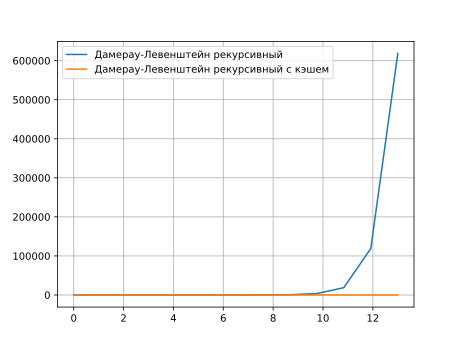
\includegraphics[scale=0.7]{graph1.png}
            \caption{Зависимость времени работы алгоритмов от длин строк}
            \label{graph:test:2}
        \end{figure}



    \section{Вывод}
        В данном разделе были поставлены эксперименты по замеру времени
        выполнения каждого из алгоритмов. Рекурсивные алгоритмы по нахождению редакционного растояния работают дольше чем матричные на несколько порядков. Время работы таких реализаций увеличивается в геометрической прогрессии. С этой проблемой помогает справляться кэширование, но такой подход увеличивает затраты в памяти. 
        
        Следовательно, матричная реализация более применима в реальных проектах.


\newpage